\documentclass[10pt]{article}

\usepackage{sbc-template}

\usepackage{graphicx,url}

\usepackage{amssymb}
\usepackage{subcaption}

%\usepackage[brazil]{babel}   
%\usepackage[latin1]{inputenc}  
\usepackage[utf8]{inputenc}  
% UTF-8 encoding is recommended by ShareLaTex

     
\sloppy

%\title{Instructions for Authors of SBC Conferences\\ Papers and Abstracts}
\title{Implementation and Analysis of Collaborative Filtering Algorithm on MovieLens Latest Small Dataset}

%\author{Luciana P. Nedel\inst{1}, Rafael H. Bordini\inst{2}, Flávio Rech
%  Wagner\inst{1}, Jomi F. Hübner\inst{3} }
\author{Xinqi Zhu 5150297, Ryan Mckay 5060961}

\address{School of Computer Science and Engineering -- University of New South Wales}
%\address{Instituto de Informática -- Universidade Federal do Rio Grande do Sul
%  (UFRGS)\\
%  Caixa Postal 15.064 -- 91.501-970 -- Porto Alegre -- RS -- Brazil
%\nextinstitute
%  Department of Computer Science -- University of Durham\\
%  Durham, U.K.
%\nextinstitute
%  Departamento de Sistemas e Computação\\
%  Universidade Regional de Blumenal (FURB) -- Blumenau, SC -- Brazil
%  \email{\{nedel,flavio\}@inf.ufrgs.br, R.Bordini@durham.ac.uk,
%  jomi@inf.furb.br}
%}


\begin{document} 

\maketitle

%\begin{abstract}
%  This meta-paper describes the style to be used in articles and short papers
%  for SBC conferences. For papers in English, you should add just an abstract
%  while for the papers in Portuguese, we also ask for an abstract in
%  Portuguese (``resumo''). In both cases, abstracts should not have more than
%  10 lines and must be in the first page of the paper.
%\end{abstract}

\begin{abstract}
We present our study of recommender system's and user-item rating systems, i.e. user-movie rating system. We focus on the most prolific algorithm in recommender systems, collaborative filtering, more specifically Latent Factor and K-Nearest-Neighbour (KNN) techniques for rating prediction and we establish a simple classification rule as a means for considering so called top N recommendations. In this report, we outline the implementation, experimentation and evaluation of our collaborative filtering solution and explore various methods to measure prediction accuracy based on experiments.
\end{abstract}

%\begin{resumo} 
%  Este meta-artigo descreve o estilo a ser usado na confecção de artigos e
%  resumos de artigos para publicação nos anais das conferências organizadas
%  pela SBC. É solicitada a escrita de resumo e abstract apenas para os artigos
%  escritos em português. Artigos em inglês deverão apresentar apenas abstract.
%  Nos dois casos, o autor deve tomar cuidado para que o resumo (e o abstract)
%  não ultrapassem 10 linhas cada, sendo que ambos devem estar na primeira
%  página do artigo.
%\end{resumo}


\section{Introduction}

Recommender system's have become very popular in recent times, implemented by many Internet giants to guide customers toward products they are likely to click on, watch, purchase or consume in general. One of the most successful recommendation algorithms is collaborative filtering.
%Recommender system has been widely used over the Internet and many Internet giants have their own version of recommender system to guide customers toward products they are more likely to be interested in. One of the most successful recommendation algorithms is collaborative filtering.

%In this project, our goal is to implement a version of collaborative filtering algorithm on a MovieLens user-movie rating dataset and do sufficient experiments to make the system work properly and give a reasonable prediction accuracy.
%
%Also we apply multiple evaluation methods to our system and see how the value of parameters change the performance of the system.

%\section{Related Work}


\section{Data Preparation}
Firstly we performed data cleaning, which included handling null values and transforming the raw data into a matrix form (movieId $\times$ userId) with new sequential indexing so that we could perform matrix factorisation and compare user and movie vectors easily. We also recorded a rated matrix which held boolean values indicating if a particular user had rated a movie.

Next we created two methods for partitioning our data random sample and temporal split. Random Sample ignores the timestamp value and takes the supplied proportion for the holdout test set as a random sample using scikit-learns ShuffleSplit. Temporal split sorts the data by timestamp and partitions the data such that the supplied proportion for the holdout set is the most recent subset of user ratings. 

The temporal split is a means of naively simulating an online recommender system as often the system will be given a new user and rating to predict at a moment in time.

\section{Implementation}

%Our implementation mainly consists of five parts, including basic Collaborative Filtering latent factor models, k-nearest-neighbor model, k-fold cross validation, ROC(receiver operating characteristic) curve and visualization.

\subsection{Collaborative Filtering Algorithm}

There are two primary areas of collaborative filtering: neighborhood methods and latent factor models\cite{MF}. Our implementation includes: 

\begin{itemize} 
	\item Latent factor model (Matrix Factorisation)
	\item KNN model
	\item K-Fold cross validation
	\item Precision-Recall Curve 
	\item Performance evaluation metrics and supporting visualizations
\end{itemize}

%Our realization of the latent factor model called matrix factorization(MF) and k-nearest-neighbor for neighborhood method.

\subsubsection{Latent Factor Model}
This algorithm will model the user-movie rating matrix as inner product of a user matrix and a movie matrix. Each movie is represented as a vector $X_i \in \mathbb{R}^f$ and each user is associated with $\theta_j \in \mathbb{R}^f$. The approximate rating by user j on movie i is:
$$\hat{r}_{ij} = X_i^T \cdot \theta_j$$

This implementation require the determination of the number of features $f$, which is used to represent the features of a movie and the preference of a user on these features. In Experimental Evaluation section we discuss the number of feature selection.

In order to get the proper $X$ and $\theta$ matrix, we use the definition of cost function from \cite{MF}:
$$J = \frac{1}{2}\sum_{(i,j):t(i,j)=1}(X_i^T \cdot \theta_j - r_{ij})^2+\frac{\lambda}{2}\sum_{i = 1}^{n_m}\sum_{k = 1}^{f}X_{ik}^{2}+\frac{\lambda}{2}\sum_{j = 1}^{n_u}\sum_{k = 1}^{f}\theta_{jk}^{2}$$
where $t(i,j)$ means movie $i$ has been rated by user $j$. $\lambda$ is the regularization coefficient and should be determined by experiment.

The gradient of $X$ and $\theta$:
$$\frac{\partial J}{\partial X_{ik}} = \sum_{j:t(i,j)=1}(X_i^T \cdot \theta_j - r_{ij})\theta_{jk}+\lambda X_{ik}$$
$$\frac{\partial J}{\partial \theta_{jk}} = \sum_{i:t(i,j)=1}(X_i^T \cdot \theta_j - r_{ij})X_{ik}+\lambda \theta_{jk}$$

Then we use the predefined optimization method of Conjugate Gradient from scipy library to train our model. In order to do so, we compress the $X$ and $\theta$ matrix into a vector to fit the minimization function.

When doing prediction, we get the inner product of $X$ and $\theta$ matrix to get $\hat{r}$ matrix. Then we replace each value in $\hat{r}$ by the nearest rating level (0.5, 1.0, 1.5 ...) and compare it with the true rating matrix $r$ (details in section 5).

\subsubsection{K-Nearest-Neighbor Model}
We explore KNN as another method of prediction based on our Latent Factor model. Using $\theta$ matrix from our Latent Factor model we compute similarity of each user in our test set to the subset of users that rated the movie that we wish to predict for the test set user.  

We compute "similarity" with two measures, Pearson Correlation and Cosine similarity as defined below.

Pearson Correlation $r_{p}$ of users $x$ and $y$ with feature vectors $r_{x}$ and $r_{y}$ respectively with $i$th feature from $\theta$ matrix.  
$$r_{p} = \dfrac{ \sum_{i\in} (r_{x,i} - \bar{r_{x}})(r_{y,i} - \bar{r_{y}})}{\sqrt{\sum_{i} (r_{x,i} - \bar{r_{x}})^{2} \sum_{i} (r_{y,i} - \bar{r_{y}})^{2}}}$$ 

Cosine Similarity is the cosine of the angle between user feature vectors x and y from $\theta$ matrix.
$$r_{c} = \cos(\textbf{x},\textbf{y}) = \frac{\sum_{i} r_{x,i} r_{y,i} }{\sqrt{\sum_{i} r_{x,i}^2} \sqrt{\sum_{i} r_{y,i}^2}} $$

From the subset of users that rated the test set movie, we select the k most similar users to the test set user by the latent features from $\theta$ matrix and the similarity measures described above. Our prediction for the test set users rating of a particular movie is the mean of the ratings given by its K nearest users. When no users had previously rated the movie from the test set, we took a simple average of all of the user in questions ratings. 

\begin{figure}[b]
    \centering
    \begin{subfigure}{0.33\textwidth}
      \centering
      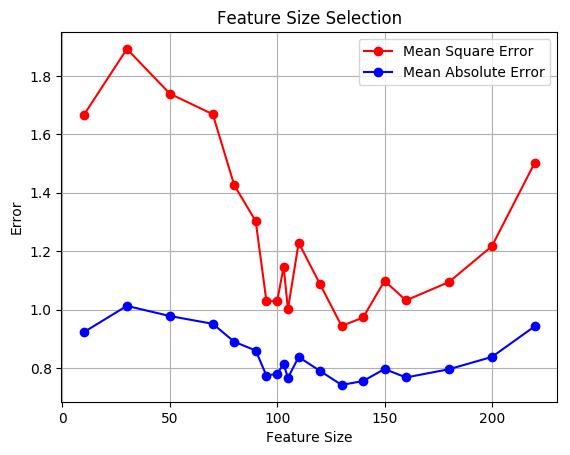
\includegraphics[width=1\textwidth]{Feature_Size_Selection}
      \caption{Feature Size Selection}
      \label{fig:Feature}
    \end{subfigure}%
    \begin{subfigure}{0.33\textwidth}
      \centering
      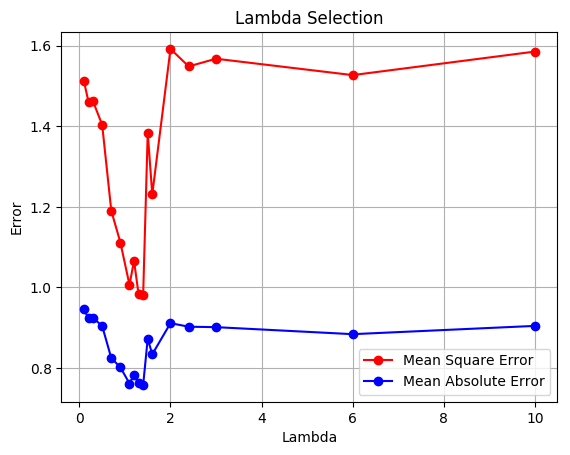
\includegraphics[width=1\textwidth]{Lambda_Selection}
      \caption{$\lambda$ Selection}
      \label{fig:Lamb}
    \end{subfigure}%
    \begin{subfigure}{0.33\textwidth}
      \centering
      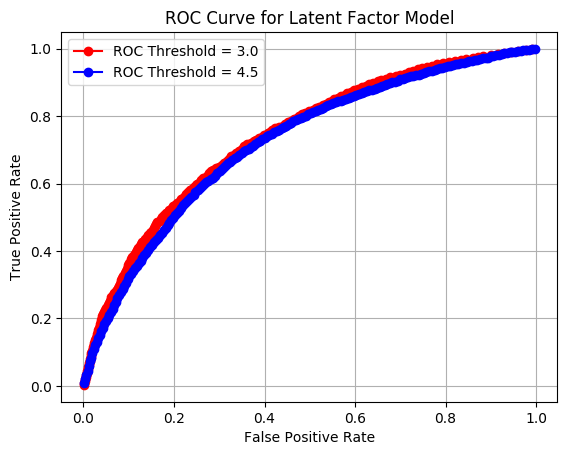
\includegraphics[width=1\textwidth]{ROC_Curve_for_Latent_Factor_Model}
      \caption{ROC Curve of Latent Factor Model}
      \label{fig:ROC}
    \end{subfigure}
\end{figure}

\subsection{K-fold Cross Validation}
We use k-fold cross validation to determine the proper number of features $f$, the regularization coefficient $\lambda$ and do any other debugging.

By using the KFold function of scikit-learns model\_selection library, we can easily split the training set into k folds and use any of them as validation set. In our implementation, we take $k=5$ and use the mean of each fold's MSE(mean square error) and MAE(mean absolute error) as final training set's and CV's MSE and MAE.

\section{Experimental Evaluation}

\subsection{Latent Factor Model}
We randomly split the raw data of user-movie rating into training set(80\%) and test set(20\%), then do experiments with k-fold cross validation with $k=5$.
The experiments include determination of the number of features $f$, regularization coefficient $\lambda$, getting learning curve and ROC curve.

Figure \ref{fig:Feature} and Figure \ref{fig:Lamb} show the  experiments to get the proper $f$ and $\lambda$ and ends up with $f=105$ and $\lambda = 1.3$. We can see when $\lambda$ is larger than 1.3 the MSE on CV set is increasing and likely to be underfitting(high bias). On the contrary, low $\lambda$ makes the system overfitting(high variance). We set $f=105$ at the elbow point because larger $f$ takes more time to train but no obvious improvement on result, and lower $f$ is not mature enough.

Figure \ref{fig:ROC} shows the ROC curve of our recommender system. The confusion matrix is defined based on the assumption that the truth rating beyond a threshold should be regarded as true positive and below as true negative\cite{CF_Recsys_Survey}. For prediction, we maintain a top rating list, i.e. top 100 rating movies to be predicted positive and rest to be predicted negative. We plot two thresholds curves, 3 and 4.5 stars. We draw the curve by changing the size of the top N list.

Figure \ref{fig:Underfitting}, Figure \ref{fig:Normal} and Figure \ref{fig:Overfitting} show the learning curves under three conditions: underfitting($\lambda = 5$), normal($\lambda = 1.3$), and overfitting($\lambda = 0.2$).

\subsection{KNN Model}
For KNN we attempted to understand if it could improve on the latent factor model by using its derived features as a measure of user similarity. We attempted a simple KNN experiment on the raw 671 user $\times$ 9066 movie matrix, but abandoned it after an extreme processing time. We would have used this result as a base line, both for our Latent Factor Model and further KNN experiments using the Latent features.

The experiments conducted with our KNN implementation were to understand the effect of the value of $k$ and the sampling method on MSE and MAE.
\begin{figure}[t]
    \centering
    \begin{subfigure}{0.33\textwidth}
      \centering
      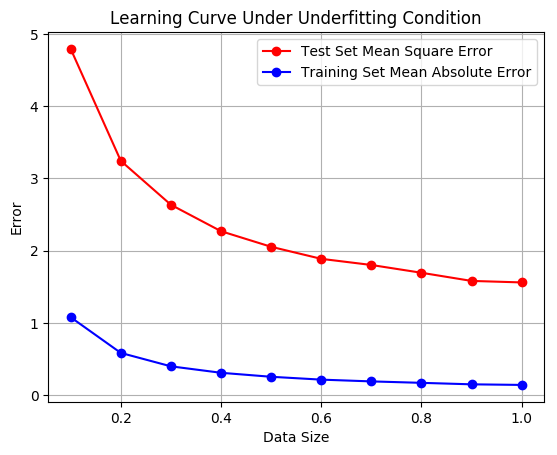
\includegraphics[width=1\textwidth]{Learning_Curve_Under_Underfitting_Condition}
      \caption{Underfitting}
      \label{fig:Underfitting}
    \end{subfigure}%
    \begin{subfigure}{0.33\textwidth}
      \centering
      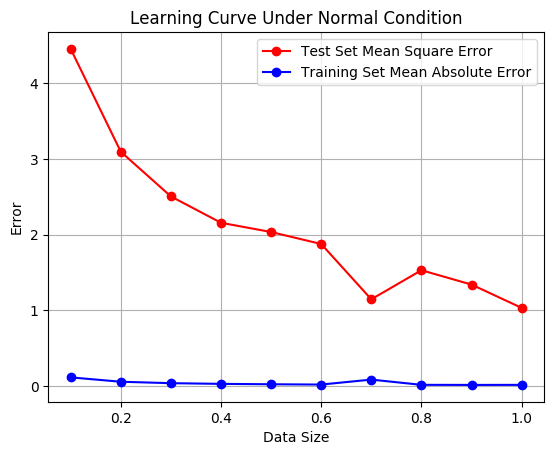
\includegraphics[width=1\textwidth]{Learning_Curve_Under_Normal_Condition}
      \caption{Normal}
      \label{fig:Normal}
    \end{subfigure}
    \begin{subfigure}{0.33\textwidth}
      \centering
      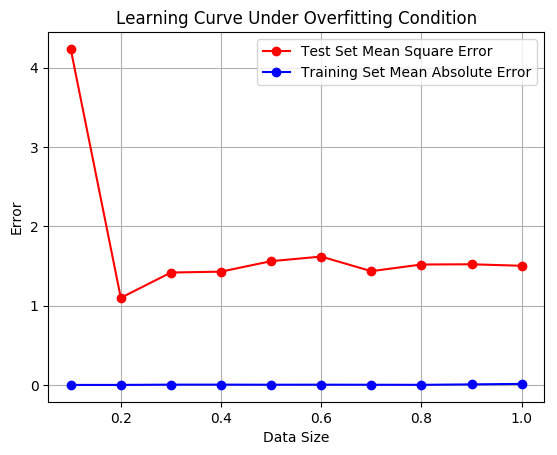
\includegraphics[width=1\textwidth]{Learning_Curve_Under_Overfitting_Condition}
      \caption{Overfitting}
      \label{fig:Overfitting}
    \end{subfigure}%
\end{figure}
%\begin{figure}[ht]
%\centering
%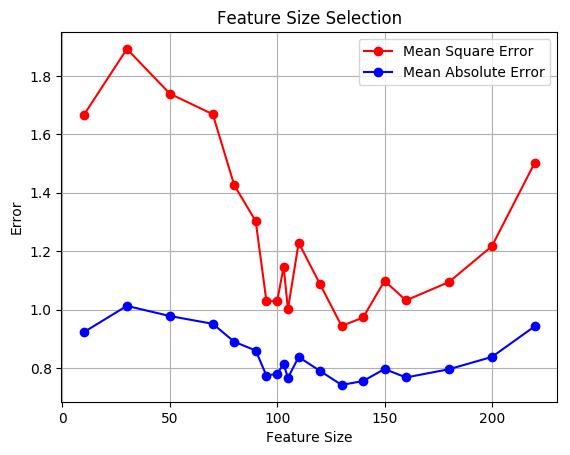
\includegraphics[width=.5\textwidth]{Feature_Size_Selection.png}
%\caption{Feature Size Selection}
%\label{fig:Feature}
%\end{figure}
%
%\begin{figure}[ht]
%\centering
%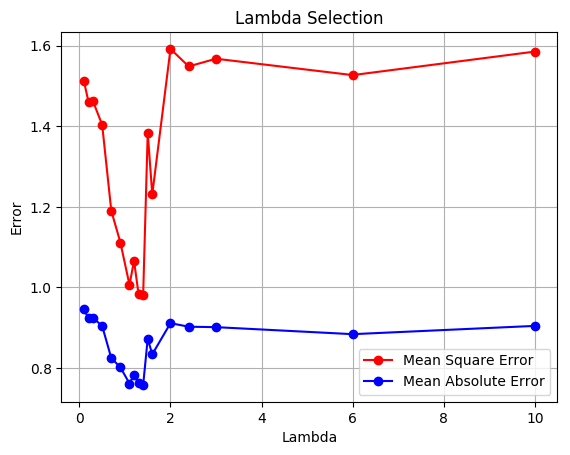
\includegraphics[width=.5\textwidth]{Lambda_Selection.png}
%\caption{$\lambda$ Selection}
%\label{fig:Lamb}
%\end{figure}

%In tables, try to avoid the use of colored or shaded backgrounds, and avoid
%thick, doubled, or unnecessary framing lines. When reporting empirical data,
%do not use more decimal digits than warranted by their precision and
%reproducibility. Table caption must be placed before the table (see Table 1)
%and the font used must also be Helvetica, 10 point, boldface, with 6 points of
%space before and after each caption.
%
%\begin{table}[ht]
%\centering
%\caption{Variables to be considered on the evaluation of interaction
%  techniques}
%\label{tab:exTable1}
%\smallskip
%\begin{tabular}{|l|c|c|}
%\hline
%& Value 1 & Value 2\\[0.5ex]
%\hline
%&&\\[-2ex]
%Case 1 & 1.0 $\pm$ 0.1 & 1.75$\times$10$^{-5}$ $\pm$ 5$\times$10$^{-7}$\\[0.5ex]
%\hline
%&&\\[-2ex]
%Case 2 & 0.003(1) & 100.0\\[0.5ex]
%\hline
%\end{tabular}
%\end{table}

\subsection{Results}

For latent factor model, with random split, our system reaches an mean square error of 0.974 and mean absolute error of 0.756. The average accuracy of very close prediction(less or equal to error of 0.5) on rated movies is 57.5\%. This is an amazing ratio because that means most of the user's interaction with movies has been correctly predicted. The ROC curve shows that the prediction is much better than randomly guess.

Because our assumption on true condition of confusion matrix is based on the movies the user has already rated, the number of movies in this set is much fewer than real condition, which means false negative is likely to be underestimated. In order to predict more accurately, we may use the user's browsing history to identify which movies are implicitly rejected by that user, such as being recommended but ignored. This will use online technique to track user's behavior and will make a better assumption of true condition and prediction condition in confusion matrix.

For KNN model using a random sample to partition the data we observed a MSE of ~1 and MAE of ~0.765 and using a temporal split of the data we observed a best MSE of ~1.16 and MAE of 0.84. We observed similar results for calculating similarity with Cosine and Pearson Correlation measures. In all cases Cosine measure was superior, particularly for lower values of $k$.

Considering the effect of $k$ on our metrics from Figures \ref{fig:knn1} - \ref{fig:knn4} we can conclude that they converge quite quickly and that $k > 10$ for the random split and $k > 5$ for the temporal split yielded no specific improvement. We should consider that with a larger dataset we will find a larger number and more specifically similar users and hence $k$ may not converge so quickly. 

In regards to the temporal split convergence we must consider the temporal distribution of the data as movies could be rated at similar, as may users rate many movies at similar times. We hypothesize that this could enhance the cold start problem producing a higher error, but also producing a quicker convergence of k as a user in the test partition may have sparse entries in the training partition and would result in inaccurate similarity scores.    

\begin{figure}[t]
    \centering
    \begin{subfigure}{0.5\textwidth}
      \centering
      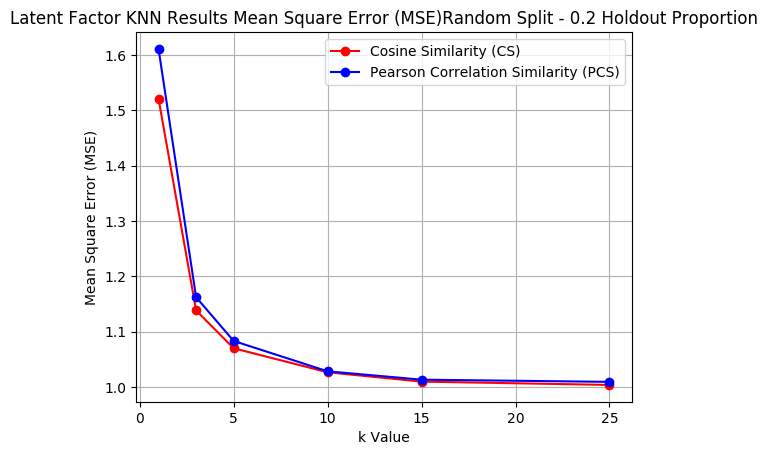
\includegraphics[width=1\textwidth]{KNN_MSE_Random_Split}
      \caption{KNN MSE Random Split}
      \label{fig:knn1}
    \end{subfigure}%
    \begin{subfigure}{0.5\textwidth}
      \centering
      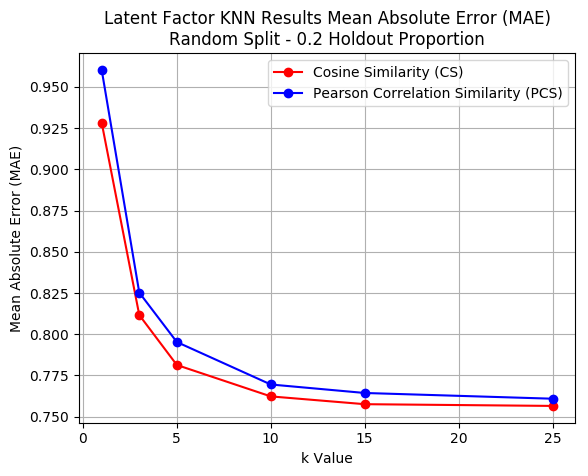
\includegraphics[width=0.8\textwidth]{KNN_MAE_Random_Split}
      \caption{KNN MAE Random Split}
      \label{fig:knn2}
    \end{subfigure}
\end{figure}
\begin{figure}[t]
	\begin{subfigure}{0.5\textwidth}
      \centering
      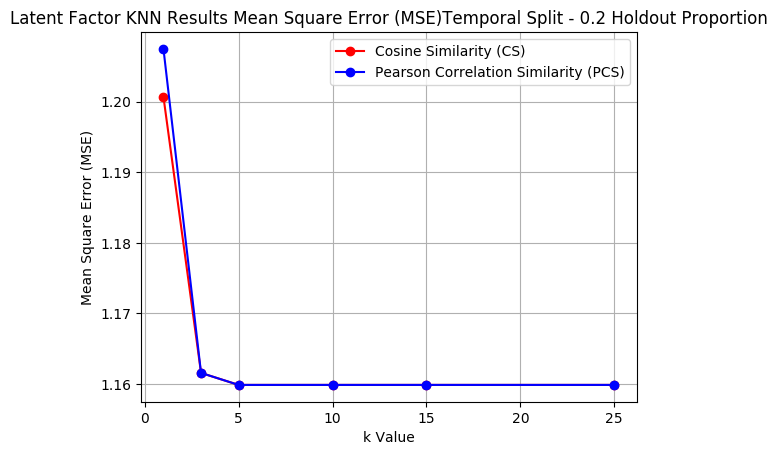
\includegraphics[width=1\textwidth]{KNN_MSE_Temporal_Split}
      \caption{KNN MSE Temporal Split}
      \label{fig:knn3}
    \end{subfigure}%
    \begin{subfigure}{0.5\textwidth}
      \centering
      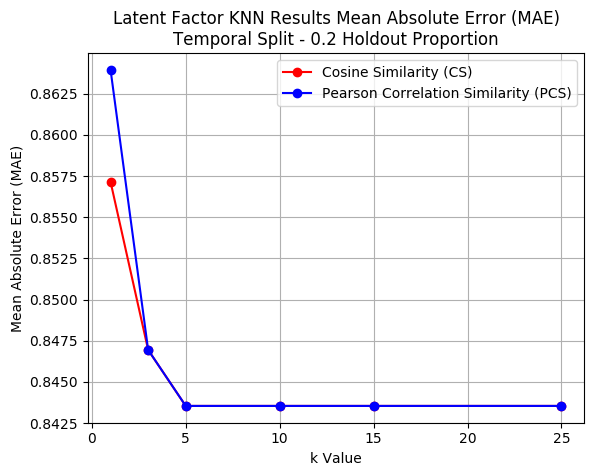
\includegraphics[width=0.8\textwidth]{KNN_MAE_Temporal_Split}
      \caption{KNN MAE Temporal Split}
      \label{fig:knn4}
    \end{subfigure}
\end{figure}

\section{Conclusion}
By implementing collaborative filtering, the most prolific set of algorithms used in recommender systems today, we sought to gain a working understanding of the nuts and bolts of what, how and why collaborative filtering is an effective recommendation and prediction tool. 

We implemented a Latent Factor Model using a matrix factorization algorithm with regularization and a KNN Model that used the Latent features derived from the matrix factorization to greatly reduce processing time over simple KNN, however its results were not superior to the Latent Factor Model. The Latent Factor Model produced impressive results considering the simplicity of its formulation with room for additional features to improve results further.

By focusing on experimentation over algorithmic implementation we have created a foundation from which we can modify and expand with clear and useful evaluation results to guide decisions in a thoughtful and quantitative manner.

%Bibliographic references must be unambiguous and uniform.  We recommend giving
%the author names references in brackets, e.g. \cite{knuth:84},
%\cite{boulic:91}, and \cite{smith:99}.
%
%The references must be listed using 12 point font size, with 6 points of space
%before each reference. The first line of each reference should not be
%indented, while the subsequent should be indented by 0.5 cm.

\bibliographystyle{unsrt}
\bibliography{sbc-template}

\end{document}
